\part{Discrete Noiseless Systems}

\section{The Discrete Noiseless Channel}
\label{sec:1}

Teletype and telegraphy are two simple examples of a discrete channel
for transmitting information.  Generally, a discrete channel will mean
a system whereby a sequence of choices from a finite set of elementary
symbols $S_1,\dots,S_n$ can be transmitted from one point to another.
Each of the symbols $S_i$ is assumed to have a certain duration in
time $t_i$ seconds (not necessarily the same for different $S_i$, for
example the dots and dashes in telegraphy).  It is not required that
all possible sequences of the $S_i$ be capable of transmission on the
system; certain sequences only may be allowed.  These will be possible
signals for the channel.  Thus in telegraphy suppose the symbols are:
(1) A dot, consisting of line closure for a unit of time and then line
open for a unit of time; (2) A dash, consisting of three time units
of closure and one unit open; (3) A letter space consisting of, say,
three units of line open; (4) A word space of six units of line open.
We might place the restriction on allowable sequences that no spaces
follow each other (for if two letter spaces are adjacent, it is
identical with a word space).  The question we now consider is how one
can measure the capacity of such a channel to transmit information.

In the teletype case where all symbols are of the same duration, and any
sequence of the 32 symbols is allowed the answer is easy.  Each symbol
represents five bits of information.  If the system transmits $n$ symbols
per second it is natural to say that the channel has a capacity of $5n$
bits per second.  This does not mean that the teletype channel will always
be transmitting information at this rate --- this is the maximum possible
rate and whether or not the actual rate reaches this maximum depends on
the source of information which feeds the channel, as will appear later.

In the more general case with different lengths of symbols and constraints
on the allowed sequences, we make the following definition:
\par\noindent Definition:
The capacity $C$ of a discrete channel is given by
$$
C = \lim_{T\to\infty} \frac{\log N(T)}{T}
$$
where $N(T)$ is the number of allowed signals of duration $T$.

It is easily seen that in the teletype case this reduces to the previous
result.  It can be shown that the limit in question will exist as a
finite number in most cases of interest.  Suppose all sequences of the
symbols $S_1,\dots,S_n$ are allowed and these symbols have durations
$t_1,\dots,t_n$.  What is the channel capacity?  If $N(t)$ represents
the number of sequences of duration $t$ we have
$$
N(t) = N(t-t_1) + N(t-t_2) + \dots + N(t-t_n).
$$
The total number is equal to the sum of the numbers of sequences ending
in $S_1,S_2,\dots,S_n$ and these are $N(t-t_1),N(t-t_2),\dots,N(t-t_n)$,
respectively.  According to a well-known result in finite differences,
$N(t)$ is then asymptotic for large $t$ to $X_0^t$ where $X_0$ is the
largest real solution of the characteristic equation:
$$
X^{-t_1} + X^{-t_2} + \dots + X^{-t_n} = 1
$$
and therefore
$$
C = \log X_0.
$$

In case there are restrictions on allowed sequences we may still
often obtain a difference equation of this type and find $C$ from the
characteristic equation.  In the telegraphy case mentioned above
$$
N(t) = N(t-2) + N(t-4) + N(t-5) + N(t-7) + N(t-8) + N(t-10)
$$
as we see by counting sequences of symbols according to the last or
next to the last symbol occurring.  Hence $C$ is $- \log \mu_0$ where
$\mu_0$ is the positive root of $1= \mu^2 + \mu^4 + \mu^5 + \mu^7 +
\mu^8 + \mu^{10}$.  Solving this we find $C= 0.539$.

A very general type of restriction which may be placed on allowed
sequences is the following: We imagine a number of possible states
$a_1,a_2,\dots,\allowbreak a_m$.  For each state only certain symbols from the
set $S_1,\dots,S_n$ can be transmitted (different subsets for the
different states).  When one of these has been transmitted the state
changes to a new state depending both on the old state and the particular
symbol transmitted.  The telegraph case is a simple example of this.
There are two states depending on whether or not a space was the last
symbol transmitted.  If so, then only a dot or a dash can be sent next
and the state always changes.  If not, any symbol can be transmitted and
the state changes if a space is sent, otherwise it remains the same.  The
conditions can be indicated in a linear graph as shown in Fig.~\ref{fig:2}.
\begin{figure}[ht]
\centerline{\begin{picture}(0,0)%
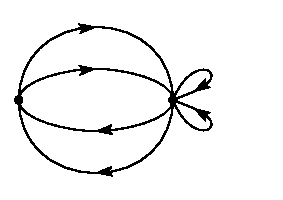
\epsfig{file=fig2.ps}%
\end{picture}%
\begin{small}%
\setlength{\unitlength}{1bp}%
\begin{picture}(120,80)
\put(100,21){\makebox(0,0){\sc dash}}
\put(100,60){\makebox(0,0){\sc dot}}
\put(38,81){\makebox(0,0){\sc dash}}
\put(38,61){\makebox(0,0){\sc dot}}
\put(38,20){\makebox(0,0){\sc letter space}}
\put(38,0){\makebox(0,0){\sc word space}}
\end{picture}%
\end{small}%
\endinput
}
\caption{Graphical representation of the constraints on telegraph symbols.}
\label{fig:2}
\end{figure}
The junction points correspond to the states and the lines indicate the
symbols possible in a state and the resulting state.  In Appendix 1 it
is shown that if the conditions on allowed sequences can be described
in this form $C$  will exist and can be calculated in accordance with
the following result:
\begin{theorem}
\label{thm:1}
Let $b_{ij}^{(s)}$ be the duration of the $s^{\text{th}}$ symbol which
is allowable in state $i$ and leads to state $j$.  Then the channel
capacity $C$ is equal to $\log W$ where $W$ is the largest real root of the
determinant equation:
$$
\Bigl| \sum_s W^{-b_{ij}^{(s)}} - \delta_{ij} \Bigr| = 0
$$
where $\delta_{ij} =1$ if $i=j$ and is zero otherwise.
\end{theorem}

For example, in the telegraph case (Fig.~\ref{fig:2}) the determinant is:
$$
\biggl| \begin{matrix}
-1 & (W^{-2} + W^{-4}) \\
(W^{-3} + W^{-6}) & (W^{-2} + W^{-4} -1 )
\end{matrix} \biggr| = 0.
$$
On expansion this leads to the equation given above for this
case.

\section{The Discrete Source of Information}

We have seen that under very general conditions the logarithm of the
number of possible signals in a discrete channel increases linearly
with time.  The capacity to transmit information can be specified by
giving this rate of increase, the number of bits per second required to
specify the particular signal used.

We now consider the information source.  How is an information source
to be described mathematically, and how much information in bits per
second is produced in a given source?  The main point at issue is the
effect of statistical knowledge about the source in reducing the required
capacity of the channel, by the use of proper encoding of the information.
In telegraphy, for example, the messages to be transmitted consist of
sequences of letters.  These sequences, however, are not completely
random.  In general, they form sentences and have the statistical
structure of, say, English.  The letter E occurs more frequently than Q,
the sequence TH more frequently than XP, etc.  The existence of this
structure allows one to make a saving in time (or channel capacity)
by properly encoding the message sequences into signal sequences.
This is already done to a limited extent in telegraphy by using the
shortest channel symbol, a dot, for the most common English letter E;
while the infrequent letters, Q, X, Z are represented by longer sequences
of dots and dashes.  This idea is carried still further in certain
commercial codes where common words and phrases are represented by four-
or five-letter code groups with a considerable saving in average time.
The standardized greeting and anniversary telegrams now in use extend
this to the point of encoding a sentence or two into a relatively short
sequence of numbers.

We can think of a discrete source as generating the message, symbol
by symbol.  It will choose successive symbols according to certain
probabilities depending, in general, on preceding choices as well as the
particular symbols in question.  A physical system, or a mathematical
model of a system which produces such a sequence of symbols governed by
a set of probabilities, is known as a stochastic process.\footnote{See,
for example, S. Chandrasekhar, ``Stochastic Problems in Physics and
Astronomy,'' {\it Reviews of Modern Physics}, v.~15, No.~1, January 1943,
p.~1.} We may consider a discrete source, therefore, to be represented by
a stochastic process.  Conversely, any stochastic process which produces
a discrete sequence of symbols chosen from a finite set may be considered
a discrete source.  This will include such cases as:
\begin{enumerate}
\item
Natural written languages such as English, German, Chinese.
\item
Continuous information sources that have been rendered discrete by some
quantizing process.
For example, the quantized speech from a PCM transmitter, or a quantized
television signal.
\item
Mathematical cases where we merely define abstractly a stochastic process
which generates a sequence of symbols.
The following are examples of this last type of source.
\begin{enumerate}
\renewcommand{\labelenumii}{(\Alph{enumii})}
\item
Suppose we have five letters A, B, C, D, E which are chosen each with
probability .2, successive choices being independent.  This would lead
to a sequence of which the following is a typical example.

B D C B C E C C C A D C B D D A A E C E E A\newline
A B B D A E E C A C E E B A E E C B C E A D.

This was constructed with the use of a table of random
numbers.\footnote{Kendall and Smith, {\it Tables of Random Sampling
Numbers,} Cambridge, 1939.}
\item
Using the same five letters let the probabilities be .4, .1, .2, .2,
.1, respectively, with successive choices independent.  A typical message
from this source is then:

A A A C D C B D C E A A D A D A C E D A\newline
E A D C A B E D A D D C E C A A A A A D.
\item
A more complicated structure is obtained if successive symbols are not
chosen independently but their probabilities depend on preceding letters.
In the simplest case of this type a choice depends only on the preceding
letter and not on ones before that.  The statistical structure can then be
described by a set of transition probabilities $p_i(j)$, the probability
that letter $i$ is followed by letter $j$.  The indices $i$ and $j$ range
over all the possible symbols.  A second equivalent way of specifying
the structure is to give the ``digram'' probabilities $p(i,j)$, i.e.,
the relative frequency of the digram $i ~j$.  The letter frequencies
$p(i)$, (the probability of letter $i$), the transition probabilities
$p_i(j)$ and the digram probabilities $p(i,j)$ are related by the
following formulas:
\begin{align*}
  p(i)&= \sum_j p(i,j) = \sum_j p(j,i) = \sum_j p(j) p_j (i) \\
p(i,j)&= p(i) p_i(j) \\
\sum_j^{\rule{0pt}{1ex}} p_i (j)&= \sum_i p(i) = \sum_{i,j} p(i,j) = 1.
\end{align*}

As a specific example suppose there are three letters A, B, C with the
probability tables:
$$
\renewcommand{\arraystretch}{1.2}
\begin{array}{r | c c c}
\multicolumn{1}{c}{p_i(j)} & \multicolumn{3}{|c}{j} \\
  & \text{A} & \text{B} & \text{C} \\ \hline
 \text{A} & 0 & \frac45 & \frac15 \\
i\quad\text{B} & \frac12 & \frac12 & 0 \\
\text{C} & \frac12 & \frac25 & \frac{1}{10}
\end{array}
\qquad
\begin{array}{c|c}
i & p(i) \\
\\
\text{A} & \frac{9}{27} \\
\text{B} & \frac{16}{27} \\
\text{C} & \frac{2}{27}
\end{array}
\qquad
\begin{array}{r | c c c}
\multicolumn{1}{c}{p(i,j)} & \multicolumn{3}{|c}{j} \\
  & \text{A} & \text{B} & \text{C} \\ \hline
\text{A} & 0 & \frac{4}{15} & \frac{1}{15} \\
i\quad\text{B} & \frac{8}{27} & \frac{8}{27} & 0 \\
\text{C} & \frac{1}{27} & \frac{4}{135} & \frac{1}{135}
\end{array}
$$
A typical message from this source is the following:

A B B A B A B A B A B A B A B B B A B B B B B A B A B A B A B A B B B A C A C A B B A B B B B A B B A B A C B B B A B A.

The next increase in complexity would involve trigram frequencies but
no more.  The choice of a letter would depend on the preceding two letters
but not on the message before that point.  A set of trigram frequencies
$p(i,j,k)$ or equivalently a set of transition probabilities $p_{ij}(k)$
would be required.  Continuing in this way one obtains successively
more complicated stochastic processes.  In the general $n$-gram case a
set of $n$-gram probabilities $p(i_1,i_2,\dots,i_n)$ or of transition
probabilities $p_{i_1,i_2,\dots,i_{n-1}}(i_n)$ is required
to specify the statistical structure.

\item
Stochastic processes can also be defined which produce a text consisting
of a sequence of ``words.'' Suppose there are five letters A, B, C, D,
E and 16 ``words'' in the language with associated probabilities:
\begin{center}
\begin{tabular}{l@{~}l l@{~}l l@{~}l l@{~}l}
.10 & A & .16 & BEBE & .11 & CABED & .04 & DEB \\
.04 & ADEB & .04 & BED & .05 & CEED & .15 & DEED \\
.05 & ADEE & .02 & BEED & .08 & DAB & .01 & EAB \\
.01 & BADD & .05 & CA & .04 & DAD & .05 & EE
\end{tabular}
\end{center}
Suppose successive ``words'' are chosen independently and are separated by
a space.  A typical message might be:

DAB EE A BEBE DEED DEB ADEE ADEE EE DEB
BEBE BEBE BEBE ADEE BED DEED DEED CEED
ADEE A DEED DEED BEBE CABED BEBE BED DAB
DEED ADEB.

If all the words are of finite length this process is equivalent to one
of the preceding type, but the description may be simpler in terms of
the word structure and probabilities.  We may also generalize here and
introduce transition probabilities between words, etc.
\end{enumerate}
\end{enumerate}

These artificial languages are useful in constructing simple problems and
examples to illustrate various possibilities.  We can also approximate
to a natural language by means of a series of simple artificial
languages.  The zero-order approximation is obtained by choosing all
letters with the same probability and independently.  The first-order
approximation is obtained by choosing successive letters independently
but each letter having the same probability that it has in the natural
language.\footnote{Letter, digram and trigram frequencies are given in
{\it Secret and Urgent\/} by Fletcher Pratt, Blue Ribbon Books, 1939.
Word frequencies are tabulated in {\it Relative Frequency of English
Speech Sounds,} G. Dewey, Harvard University Press, 1923.} Thus, in the
first-order approximation to English, E is chosen with probability .12
(its frequency in normal English) and W with probability~.02, but there
is no influence between adjacent letters and no tendency to form the
preferred digrams such as TH, ED, etc.  In the second-order approximation,
digram structure is introduced.  After a letter is chosen, the next one is
chosen in accordance with the frequencies with which the various letters
follow the first one.  This requires a table of digram frequencies $p_i(j)$.
In the third-order approximation, trigram structure is introduced.  Each
letter is chosen with probabilities which depend on the preceding two
letters.

\section{The Series of Approximations to English}

To give a visual idea of how this series of processes approaches a
language, typical sequences in the approximations to English have been
constructed and are given below.  In all cases we have assumed a 27-symbol
``alphabet,'' the 26 letters and a space.
\begin{enumerate}
\item
Zero-order approximation (symbols independent and equiprobable).
\begin{quote}
\sloppy
XFOML RXKHRJFFJUJ ZLPWCFWKCYJ FFJEYVKCQSGHYD QPA\-AMKBZ\-A\-AC\-IB\-ZL\-HJQD.
\end{quote}
\item
First-order approximation (symbols independent but with frequencies of
English text).
\begin{quote}
\sloppy
OCRO HLI RGWR NMIELWIS EU LL NBNESEBYA TH EEI ALHENHTTPA OOBTTVA NAH BRL.
\end{quote}
\item
Second-order approximation (digram structure as in English).
\begin{quote}
\sloppy
ON IE ANTSOUTINYS ARE T INCTORE ST BE S DEAMY ACHIN D ILONASIVE TUCOOWE
AT TEASONARE FUSO TIZIN ANDY TOBE SEACE CTISBE.
\end{quote}
\item
Third-order approximation (trigram structure as in English).
\begin{quote}
\sloppy
IN NO IST LAT WHEY CRATICT FROURE BIRS GROCID PONDENOME OF DEMONSTURES
OF THE REPTAGIN IS REGOACTIONA OF CRE.
\end{quote}
\item
First-order word approximation.  Rather than continue with tetragram,
\dots, $n$-gram structure it is easier and better to jump at this
point to word units.  Here words are chosen independently but with their
appropriate frequencies.
\begin{quote}
\sloppy
REPRESENTING AND SPEEDILY IS AN GOOD APT OR COME CAN DIFFERENT NATURAL
HERE HE THE A IN CAME THE TO OF TO EXPERT GRAY COME TO FURNISHES THE
LINE MESSAGE HAD BE THESE.
\end{quote}
\item
Second-order word approximation.  The word transition probabilities are
correct but no further structure is included.
\begin{quote}
\sloppy
THE HEAD AND IN FRONTAL ATTACK ON AN ENGLISH WRITER THAT THE CHARACTER
OF THIS POINT IS THEREFORE ANOTHER METHOD FOR THE LETTERS THAT THE TIME
OF WHO EVER TOLD THE PROBLEM FOR AN UNEXPECTED.
\end{quote}
\end{enumerate}

The resemblance to ordinary English text increases quite noticeably
at each of the above steps.  Note that these samples have reasonably
good structure out to about twice the range that is taken into account
in their construction.  Thus in (3) the statistical process insures
reasonable text for two-letter sequences, but four-letter sequences from
the sample can usually be fitted into good sentences.  In (6) sequences
of four or more words can easily be placed in sentences without unusual or
strained constructions.  The particular sequence of ten words ``attack on
an English writer that the character of this'' is not at all unreasonable.
It appears then that a sufficiently complex stochastic process will give
a satisfactory representation of a discrete source.

The first two samples were constructed by the use of a book of random
numbers in conjunction with (for example 2) a table of letter frequencies.
This method might have been continued for (3), (4) and (5), since digram,
trigram and word frequency tables are available, but a simpler equivalent
method was used.  To construct (3) for example, one opens a book at random
and selects a letter at random on the page.  This letter is recorded.
The book is then opened to another page and one reads until this letter
is encountered.  The succeeding letter is then recorded.  Turning to
another page this second letter is searched for and the succeeding
letter recorded, etc.  A similar process was used for (4), (5) and (6).
It would be interesting if further approximations could be constructed,
but the labor involved becomes enormous at the next stage.

\section{Graphical Representation of a Markoff Process}

Stochastic processes of the type described above are known mathematically
as discrete Markoff processes and have been extensively studied in
the literature.\footnote{For a detailed treatment see M. Fr\'echet,
{\it M\'ethode des fonctions arbitraires.  Th\'eorie des \'ev\'enements
en cha\^{\i}ne dans le cas d'un nombre fini d'\'etats possibles}.  Paris,
Gauthier-Villars, 1938.} The general case can be described as follows:
There exist a finite number of possible ``states'' of a system;
$S_1,S_2,\dots,S_n$.  In addition there is a set of transition
probabilities; $p_i(j)$ the probability that if the system is in state $S_i$
it will next go to state $S_j$.  To make this Markoff process into an
information source we need only assume that a letter is produced for each
transition from one state to another.  The states will correspond to the
``residue of influence'' from preceding letters.

The situation can be represented graphically as shown in
Figs.~\ref{fig:3}, \ref{fig:4} and \ref{fig:5}.
\begin{figure}[ht]
\centerline{\begin{picture}(0,0)%
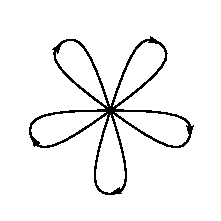
\epsfig{file=fig3.ps}%
\end{picture}%
\begin{small}%
\setlength{\unitlength}{1bp}%
\begin{picture}(90,90)
\put(37,80){\makebox(0,0){\sc a}}
\put(77,70){\makebox(0,0){\sc b}}
\put(89,30){\makebox(0,0){\sc c}}
\put(36,1){\makebox(0,0){\sc d}}
\put(3,43){\makebox(0,0){\sc e}}
\put(0,30){\makebox(0,0){\sf .1}}
\put(50,75){\makebox(0,0){\sf .1}}
\put(90,43){\makebox(0,0){\sf .2}}
\put(53,0){\makebox(0,0){\sf .2}}
\put(10,70){\makebox(0,0){\sf .4}}
\end{picture}%
\end{small}%
\endinput
}
\caption{A graph corresponding to the source in example B.}
\label{fig:3}
\end{figure}
The ``states'' are the junction points in the graph and the probabilities
and letters produced for a transition are given beside the corresponding
line.  Figure~\ref{fig:3} is for the example B in Section 2, while
Fig.~\ref{fig:4} corresponds to the example C\@.
\begin{figure}[ht]
\centerline{\begin{picture}(0,0)%
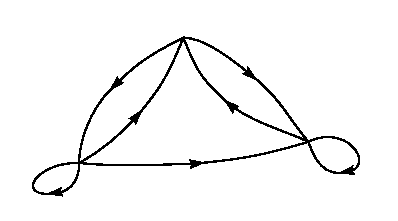
\epsfig{file=fig4.ps}%
\end{picture}%
\setlength{\unitlength}{1bp}%
\begin{small}%
\begin{picture}(175,90)
\put(85,60){\makebox(0,0){\sc a}}
\put(70,50){\makebox(0,0){\sc a}}
\put(110,72){\makebox(0,0){\sc b}}
\put(167,29){\makebox(0,0){\sc b}}
\put(48,13){\makebox(0,0){\sc b}}
\put(4,15){\makebox(0,0){\sc c}}
\put(51,70){\makebox(0,0){\sc c}}
\put(4,3){\makebox(0,0){\sf .1}}
\put(56,34){\makebox(0,0){\sf .5}}
\put(105,38){\makebox(0,0){\sf .5}}
\put(167,14){\makebox(0,0){\sf .5}}
\put(31,48){\makebox(0,0){\sf .2}}
\put(129,55){\makebox(0,0){\sf .8}}
\put(104,16){\makebox(0,0){\sf .4}}
\end{picture}%
\end{small}%
\endinput
}
\caption{A graph corresponding to the source in example C.}
\label{fig:4}
\end{figure}
In Fig.~\ref{fig:3} there is only one state since successive letters are
independent.  In Fig.~\ref{fig:4} there are as many states as letters.
If a trigram example were constructed there would be at most $n^2$
states corresponding to the possible pairs of letters preceding the
one being chosen.  Figure~\ref{fig:5} is a graph for the case of word
structure in example D\@.  Here S corresponds to the ``space'' symbol.

\section{Ergodic and Mixed Sources}
As we have indicated above a discrete source for our purposes can be
considered to be represented by a Markoff process.  Among the possible
discrete Markoff processes there is a group with special properties of
significance in communication theory.  This special class consists of the
``ergodic'' processes and we shall call the corresponding sources ergodic
sources.  Although a rigorous definition of an ergodic process is somewhat
involved, the general idea is simple.  In an ergodic process every
sequence produced by the process is the same in statistical properties.
Thus the letter frequencies, digram frequencies, etc., obtained from
particular sequences, will, as the lengths of the sequences increase,
approach definite limits independent of the particular sequence.
Actually this is not true of every sequence but the set for which it
is false has probability zero.  Roughly the ergodic property means
statistical homogeneity.

All the examples of artificial languages given above are ergodic.
This property is related to the structure of the corresponding graph.
If the graph has the following two properties\footnote{These are
restatements in terms of the graph of conditions given in Fr\'echet.}
the corresponding process will be ergodic:
\begin{enumerate}
\item
The graph does not consist of two isolated parts A and B such that it
is impossible to go from junction points in part A to junction points
in part B along lines of the graph in the direction of arrows and also
impossible to go from junctions in part B to junctions in part A.
\item
A closed series of lines in the graph with all arrows on the lines
pointing in the same orientation will be called a ``circuit.''
The ``length'' of a circuit is the number of lines in it.  Thus in
Fig.~\ref{fig:5} series BEBES is a circuit of length 5.  The second
property required is that the greatest common divisor of the lengths of
all circuits in the graph be one.
\end{enumerate}

\begin{figure}[ht]
\centerline{\begin{picture}(0,0)%
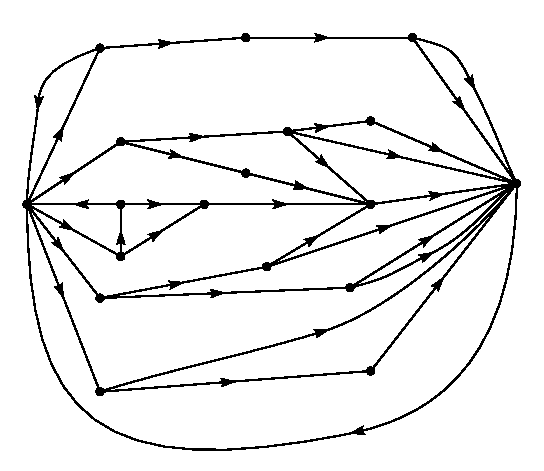
\epsfig{file=fig5.ps}%
\end{picture}%
\setlength{\unitlength}{1bp}%
\begin{small}%
\begin{picture}(245,210)
\put(6,160){\makebox(0,0){\sc s}}
\put(40,124){\makebox(0,0){\sc s}}
\put(114,8){\makebox(0,0){\sc s}}
\put(27,159){\makebox(0,0){\sc a}}
\put(125,41){\makebox(0,0){\sc a}}
\put(46,109){\makebox(0,0){\sc a}}
\put(100,142){\makebox(0,0){\sc a}}
\put(110,82){\makebox(0,0){\sc a}}
\put(22,137){\makebox(0,0){\sc b}}
\put(74,124){\makebox(0,0){\sc b}}
\put(152,162){\makebox(0,0){\sc b}}
\put(221,185){\makebox(0,0){\sc b}}
\put(200,72){\makebox(0,0){\sc b}}
\put(161,100){\makebox(0,0){\sc b}}
\put(185,100){\makebox(0,0){\sc b}}
\put(35,108){\makebox(0,0){\sc c}}
\put(33,91){\makebox(0,0){\sc d}}
\put(56,201){\makebox(0,0){\sc d}}
\put(128,135){\makebox(0,0){\sc d}}
\put(175,80){\makebox(0,0){\sc d}}
\put(172,150){\makebox(0,0){\sc d}}
\put(183,126){\makebox(0,0){\sc d}}
\put(24,60){\makebox(0,0){\sc e}}
\put(85,88){\makebox(0,0){\sc e}}
\put(141,108){\makebox(0,0){\sc e}}
\put(111,124){\makebox(0,0){\sc e}}
\put(160,135){\makebox(0,0){\sc e}}
\put(175,204){\makebox(0,0){\sc e}}
\put(198,181){\makebox(0,0){\sc e}}
\put(78,156){\makebox(0,0){\sc e}}
\put(76,107){\makebox(0,0){\sc e}}
\put(190,157){\makebox(0,0){\sc e}}
\put(120,56){\makebox(0,0){\sc e}}
\end{picture}%
\end{small}%
\endinput
}
\caption{A graph corresponding to the source in example D.}
\label{fig:5}
\end{figure}

If the first condition is satisfied but the second one violated by
having the greatest common divisor equal to $d>1$, the sequences have a
certain type of periodic structure.  The various sequences fall into $d$
different classes which are statistically the same apart from a shift
of the origin (i.e., which letter in the sequence is called letter 1).
By a shift of from 0 up to $d-1$ any sequence can be made statistically
equivalent to any other.  A simple example with $d=2$ is the following:
There are three possible letters $a,b,c$.  Letter $a$ is followed with
either $b$ or $c$ with probabilities $\frac13$ and $\frac23$
respectively.  Either $b$ or $c$ is always followed by letter $a$.
Thus a typical sequence is
$$
\text{\itshape a b a c a c a c a b a c a b a b a c a c}.
$$
This type of situation is not of much importance for our work.

If the first condition is violated the graph may be separated into a set
of subgraphs each of which satisfies the first condition.  We will assume
that the second condition is also satisfied for each subgraph.  We have
in this case what may be called a ``mixed'' source made up of a number
of pure components.  The components correspond to the various subgraphs.
If $L_1$, $L_2$, $L_3,\dots$ are the component sources we may write
$$
L = p_1 L_1 + p_2 L_2 + p_3 L_3 + \dotsb
$$
where $p_i$ is the probability of the component source $L_i$.

Physically the situation represented is this: There are several different
sources $L_1$, $L_2$, $L_3,\dots$ which are each of homogeneous statistical
structure (i.e., they are ergodic).  We do not know \emph{a priori} which
is to be used, but once the sequence starts in a given pure component
$L_i$, it continues indefinitely according to the statistical structure
of that component.

As an example one may take two of the processes defined above and assume
$p_1 = .2$ and $p_2 = .8$.  A sequence from the mixed source
$$
L=.2 L_1 + .8L_2
$$
would be obtained by choosing first $L_1$ or $L_2$ with probabilities
.2 and .8 and after this choice generating a sequence from whichever
was chosen.

Except when the contrary is stated we shall assume a source to be ergodic.
This assumption enables one to identify averages along a sequence with
averages over the ensemble of possible sequences (the probability of
a discrepancy being zero).  For example the relative frequency of the
letter A in a particular infinite sequence will be, with probability one,
equal to its relative frequency in the ensemble of sequences.

If $P_i$ is the probability of state $i$ and $p_i(j)$ the transition
probability to state $j$, then for the process to be stationary it is
clear that the $P_i$ must satisfy equilibrium conditions:
$$
P_j = \sum_i P_i p_i (j).
$$
In the ergodic case it can be shown that with any starting conditions
the probabilities $P_j(N)$ of being in state $j$ after $N$ symbols,
approach the equilibrium values as $N\to\infty$.

\section{Choice, Uncertainty and Entropy}

We have represented a discrete information source as a Markoff process.
Can we define a quantity which will measure, in some sense, how much
information is ``produced'' by such a process, or better, at what rate
information is produced?

Suppose we have a set of possible events whose probabilities of occurrence
are $p_1,p_2,\dots,p_n$.  These probabilities are known but that is
all we know concerning which event will occur.  Can we find a measure
of how much ``choice'' is involved in the selection of the event or of
how uncertain we are of the outcome?

If there is such a measure, say $H(p_1,p_2,\dots,p_n)$, it is reasonable
to require of it the following properties:
\begin{enumerate}
\item
\label{cond:1}
$H$ should be continuous in the $p_i$.
\item
\label{cond:2}
If all the $p_i$ are equal, $p_i = \frac1n$, then $H$ should be a
monotonic increasing function of $n$.  With equally likely events there
is more choice, or uncertainty, when there are more possible events.
\item
\label{cond:3}
If a choice be broken down into two successive choices, the original $H$
should be the weighted sum of the individual values of $H$.  The meaning
of this is illustrated in Fig.~\ref{fig:6}.
\begin{figure}[ht]
\centerline{\begin{picture}(0,0)%
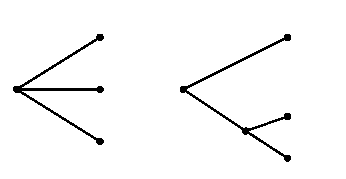
\epsfig{file=fig6.ps}%
\end{picture}%
\setlength{\unitlength}{1bp}%
\begin{small}%
\begin{picture}(150,70)
\put(25,59){\makebox(0,0){\sf 1/2}}
\put(25,41){\makebox(0,0){\sf 1/3}}
\put(22,12){\makebox(0,0){\sf 1/6}}
\put(95,51){\makebox(0,0){\sf 1/2}}
\put(95,16){\makebox(0,0){\sf 1/2}}
\put(118,25){\makebox(0,0){\sf 2/3}}
\put(114,3){\makebox(0,0){\sf 1/3}}
\put(140,60){\makebox(0,0){\sf 1/2}}
\put(140,22){\makebox(0,0){\sf 1/3}}
\put(140,2){\makebox(0,0){\sf 1/6}}
\end{picture}%
\end{small}%
\endinput
}
\caption{Decomposition of a choice from three possibilities.}
\label{fig:6}
\end{figure}
At the left we have three possibilities $p_1 = \frac12$, $p_2
= \frac13$, $p_3 = \frac16$.  On the right we first choose
between two possibilities each with probability $\frac12$, and if
the second occurs make another choice with probabilities $\frac23$,
$\frac13$.  The final results have the same probabilities as before.
We require, in this special case, that
$$
H(\tfrac12,\tfrac13,\tfrac16)=H(\tfrac12,\tfrac12)
	+\tfrac12 H(\tfrac23,\tfrac13).
$$
The coefficient $\frac12$ is because
this second choice only occurs half the time.
\end{enumerate}

In Appendix~\ref{ap:2}, the following result is established:
\begin{theorem}
\label{thm:2}
The only $H$ satisfying the three above assumptions is of the form:
$$
H = - K \sum_{i=1}^n p_i \log p_i
$$
where $K$ is a positive constant.
\end{theorem}

This theorem, and the assumptions required for its proof, are in no way
necessary for the present theory.  It is given chiefly to lend a certain
plausibility to some of our later definitions.  The real justification
of these definitions, however, will reside in their implications.

Quantities of the form $H\! =\! -\! \sum p_i \log p_i$ (the constant $K$
merely amounts to a choice of a unit of measure) play a central role in
information theory as measures of information, choice and uncertainty.
The form of $H$ will be recognized as that of entropy as defined
in certain formulations of statistical mechanics\footnote{See, for
example, R. C. Tolman, {\it Principles of Statistical Mechanics,}
Oxford, Clarendon, 1938.} where $p_i$ is the probability of a system
being in cell $i$ of its phase space.  $H$ is then, for example, the $H$
in Boltzmann's famous $H$ theorem.  We shall call $H = - \sum p_i \log
p_i$ the entropy of the set of probabilities $p_1,\dots,p_n$.  If $x$
is a chance variable we will write $H(x)$ for its entropy; thus $x$ is
not an argument of a function but a label for a number, to differentiate
it from $H(y)$ say, the entropy of the chance variable $y$.

The entropy in the case of two possibilities with probabilities $p$
and $q= 1-p$, namely
$$
H = - (p \log p + q \log q)
$$
is plotted in Fig.~\ref{fig:7} as a function of $p$.
\begin{figure}[ht]
\centerline{\begin{picture}(0,0)%
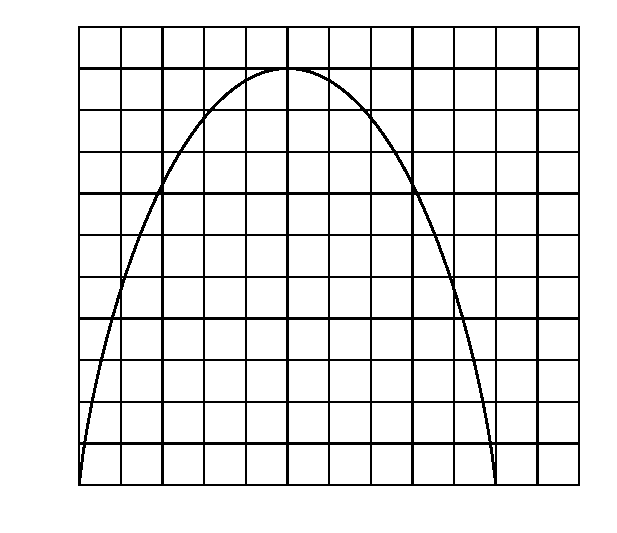
\epsfig{file=fig7.ps}%
\end{picture}%
\setlength{\unitlength}{1bp}%
\begin{small}%
\begin{picture}(280,240)
\put(0,140){\makebox(0,0){\footnotesize $H$}}
\put(0,132){\makebox(0,0){\sc bits}}
\put(140,0){\makebox(0,-2){\footnotesize $p$}}
\put(25,15){\makebox(0,0)[r]{\sf 0}}
\put(25,35){\makebox(0,0)[r]{\sf .1}}
\put(25,55){\makebox(0,0)[r]{\sf .2}}
\put(25,75){\makebox(0,0)[r]{\sf .3}}
\put(25,95){\makebox(0,0)[r]{\sf .4}}
\put(25,115){\makebox(0,0)[r]{\sf .5}}
\put(25,135){\makebox(0,0)[r]{\sf .6}}
\put(25,155){\makebox(0,0)[r]{\sf .7}}
\put(25,175){\makebox(0,0)[r]{\sf .8}}
\put(25,195){\makebox(0,0)[r]{\sf .9}}
\put(25,215){\makebox(0,0)[r]{\sf 1.0}}
\put(30,12){\makebox(0,0)[t]{\sf 0}}
\put(50,12){\makebox(0,0)[t]{\sf .1}}
\put(70,12){\makebox(0,0)[t]{\sf .2}}
\put(90,12){\makebox(0,0)[t]{\sf .3}}
\put(110,12){\makebox(0,0)[t]{\sf .4}}
\put(130,12){\makebox(0,0)[t]{\sf .5}}
\put(150,12){\makebox(0,0)[t]{\sf .6}}
\put(170,12){\makebox(0,0)[t]{\sf .7}}
\put(190,12){\makebox(0,0)[t]{\sf .8}}
\put(210,12){\makebox(0,0)[t]{\sf .9}}
\put(230,12){\makebox(0,0)[t]{\sf 1.0}}
\end{picture}%
\end{small}%
\endinput
}
\caption{Entropy in the case of two possibilities with probabilities
$p$ and $(1-p)$.}
\label{fig:7}
\end{figure}

The quantity $H$ has a number of interesting properties which further
substantiate it as a reasonable measure of choice or information.

1. $H=0$ if and only if all the $p_i$ but one are zero, this one having
the value unity.  Thus only when we are certain of the outcome does
$H$ vanish.  Otherwise $H$ is positive.

2. For a given $n$, $H$ is a maximum and equal to $\log n$ when all the
$p_i$ are equal (i.e., $\frac1n$).  This is also intuitively the most
uncertain situation.

3. Suppose there are two events, $x$ and $y$, in question with $m$
possibilities for the first and $n$ for the second.  Let $p(i,j)$ be
the probability of the joint occurrence of $i$ for the first and $j$ for
the second.  The entropy of the joint event is
$$
H(x,y) = - \sum_{i,j} p(i,j) \log p(i,j)
$$
while
\begin{align*}
H(x) &= - \sum_{i,j} p(i,j) \log \sum_j p(i,j) \\
H(y) &= - \sum_{i,j} p(i,j) \log \sum_i p(i,j).
\end{align*}
It is easily shown that
$$
H(x,y) \le H(x) + H(y)
$$
with equality only if the events are independent (i.e., $p(i,j) = p(i)
p(j)$).  The uncertainty of a joint event is less than or equal to the
sum of the individual uncertainties.

4. Any change toward equalization of the probabilities $p_1,p_2,\dots,
p_n$ increases $H$.  Thus if $p_1 < p_2$ and we increase $p_1$, decreasing
$p_2$ an equal amount so that $p_1$ and $p_2$ are more nearly equal,
then $H$ increases.  More generally, if we perform any ``averaging''
operation on the $p_i$ of the form
$$
p'_i = \sum_j a_{ij} p_j
$$
where $\sum_i a_{ij} = \sum_j a_{ij}=1$, and all $a_{ij} \ge 0$, then $H$
increases (except in the special case where this transformation amounts
to no more than a permutation of the $p_j$ with $H$ of course remaining
the same).

5. Suppose there are two chance events $x$ and $y$ as in 3, not
necessarily independent.  For any particular value $i$ that $x$ can assume
there is a conditional probability $p_i(j)$ that $y$ has the value $j$.
This is given by
$$
p_i(j)=\frac{p(i,j)}{\sum_j p(i,j)}.
$$
We define the \emph{conditional entropy} of $y$, $H_x(y)$ as the average
of the entropy of $y$ for each value of $x$, weighted according to the
probability of getting that particular $x$.  That is
$$
H_x(y) = - \sum_{i,j} p(i,j) \log p_i(j) \, .
$$
This quantity measures how uncertain we are of $y$ on the average when
we know $x$.  Substituting the value of $p_i (j)$ we obtain
\begin{align*}
H_x(y) &= - \sum_{i,j} p(i,j) \log p(i,j)
	 + \sum_{i,j} p(i,j) \log \sum_j p(i,j) \\
&= H(x,y) - H(x)
\end{align*}
or
$$
H(x,y) = H(x) + H_x (y).
$$
The uncertainty (or entropy) of the joint event $x,y$ is the uncertainty
of $x$ plus the uncertainty of $y$ when $x$ is known.

6. From 3 and 5 we have
$$
H(x) + H(y) \ge H(x,y) = H(x) + H_x(y).
$$
Hence
$$
H(y) \ge H_x (y).
$$
The uncertainty of $y$ is never increased by knowledge of $x$.  It will
be decreased unless $x$ and $y$ are independent events, in which case
it is not changed.

\section{The Entropy of an Information Source}

Consider a discrete source of the finite state type considered above.
For each possible state $i$ there will be a set of probabilities $p_i
(j)$ of producing the various possible symbols $j$.  Thus there is an
entropy $H_i$ for each state.  The entropy of the source will be defined
as the average of these $H_i$ weighted in accordance with the probability
of occurrence of the states in question:
\begin{align*}
H &= \sum_i P_i H_i \\
  &= - \sum_{i,j} P_i p_i (j) \log p_i (j) \, .
\end{align*}
This is the entropy of the source per symbol of text.  If the Markoff
process is proceeding at a definite time rate there is also an entropy
per second
$$
H' = \sum_i f_i H_i
$$
where $f_i$ is the average frequency (occurrences per second) of
state $i$.  Clearly
$$
H' = mH
$$
where $m$ is the average number of symbols produced per second.  $H$
or $H'$ measures the amount of information generated by the source per
symbol or per second.  If the logarithmic base is 2, they will represent
bits per symbol or per second.

If successive symbols are independent then $H$ is simply $- \sum p_i
\log p_i$ where $p_i$ is the probability of symbol $i$.  Suppose in
this case we consider a long message of $N$ symbols.  It will contain
with high probability about $p_1 N$ occurrences of the first symbol,
$p_2 N$ occurrences of the second, etc.  Hence the probability of this
particular message will be roughly
$$
p= p_1^{p_1 N} p_2^{p_2 N} \dotsm p_n^{p_n N}
$$
or
\begin{align*}
\log p &\doteq N \sum_i p_i \log p_i\\
\log p & \doteq - N H \\
H & \doteq \frac{\log 1/p}{N}.
\end{align*}
$H$ is thus approximately the logarithm of the reciprocal probability of
a typical long sequence divided by the number of symbols in the sequence.
The same result holds for any source.  Stated more precisely we have
(see Appendix~\ref{ap:3}):

\begin{theorem}
\label{thm:3}
Given any $\eps > 0$ and $\delta > 0$, we can find an $N_0$ such that
the sequences of any length $N \ge N_0$ fall into two classes:
\begin{enumerate}
\item
A set whose total probability is less than $\eps$.
\item
The remainder, all of whose members have probabilities satisfying the
inequality
\end{enumerate}
$$
\biggl| \frac{\log p^{-1}}{N} - H \biggr| < \delta.
$$
\end{theorem}
In other words we are almost certain to have $\dfrac{\log p^{-1}}{N}$
very close to $H$ when $N$ is large.

A closely related result deals with the number of sequences of various
probabilities.  Consider again the sequences of length $N$ and let them
be arranged in order of decreasing probability.  We define $n(q)$ to be
the number we must take from this set starting with the most probable
one in order to accumulate a total probability $q$ for those taken.
\begin{theorem}
\label{thm:4}
$$
\lim_{N\to\infty} \frac{\log n(q)}{N} = H
$$
when $q$ does not equal $0$ or $1$.
\end{theorem}

We may interpret $\log n(q)$ as the number of bits required to specify
the sequence when we consider only the most probable sequences with a
total probability $q$.  Then $\dfrac{\log n(q)}{N}$ is the number of bits
per symbol for the specification.  The theorem says that for large $N$
this will be independent of $q$ and equal to $H$.  The rate of growth of
the logarithm of the number of reasonably probable sequences is given
by $H$, regardless of our interpretation of ``reasonably probable.''
Due to these results, which are proved in Appendix 3, it is possible
for most purposes to treat the long sequences as though there were just
$2^{HN}$ of them, each with a probability $2^{-HN}$.

The next two theorems show that $H$ and $H'$ can be determined by limiting
operations directly from the statistics of the message sequences, without
reference to the states and transition probabilities between states.

\begin{theorem}
\label{thm:5}
Let $p(B_i)$ be the probability of a sequence $B_i$ of symbols from
the source.  Let
$$
G_N = - \frac1N \sum_i p(B_i) \log p(B_i)
$$
where the sum is over all sequences $B_i$ containing $N$ symbols.
Then $G_N$ is a monotonic decreasing function of $N$ and
$$
\lim_{N\to\infty} G_N = H.
$$
\end{theorem}

\begin{theorem}
\label{thm:6}
Let $p(B_i , S_j)$ be the probability of sequence $B_i$ followed by
symbol $S_j$ and $p_{B_i}(S_j) = p(B_i,S_j)/p(B_i)$ be the conditional
probability of $S_j$ after $B_i$.  Let
$$
F_N = - \sum_{i,j} p(B_i,S_j) \log p_{B_i}(S_j)
$$
where the sum is over all blocks $B_i$ of $N-1$ symbols and over all
symbols $S_j$.  Then $F_N$ is a monotonic decreasing function of $N$,
\begin{align*}
F_N &= N G_N - (N-1) G_{N-1}, \\
G_N &= \frac1N \sum_{n=1}^N F_n, \\
F_N &\le G_N,
\end{align*}
and $\lim_{N\to\infty} F_N = H$.
\end{theorem}

These results are derived in Appendix~\ref{ap:3}.  They show that a
series of approximations to $H$ can be obtained by considering only the
statistical structure of the sequences extending over $1,2,\dots,N$
symbols.  $F_N$ is the better approximation.  In fact $F_N$ is the
entropy of the $N^{\text{th}}$ order approximation to the source of the
type discussed above.  If there are no statistical influences extending
over more than $N$ symbols, that is if the conditional probability of the
next symbol knowing the preceding $(N-1)$ is not changed by a knowledge
of any before that, then $F_N = H$.  $F_N$ of course is the conditional
entropy of the next symbol when the $(N-1)$ preceding ones are known,
while $G_N$ is the entropy per symbol of blocks of $N$ symbols.

The ratio of the entropy of a source to the maximum value it could
have while still restricted to the same symbols will be called its
\emph{relative entropy}.  This is the maximum
compression possible when we encode into the same alphabet.  One minus
the relative entropy is the \emph{redundancy}.  The redundancy of ordinary
English, not considering statistical structure over greater distances
than about eight letters, is roughly 50\%.  This means that when we
write English half of what we write is determined by the structure of
the language and half is chosen freely.  The figure 50\% was found by
several independent methods which all gave results in this neighborhood.
One is by calculation of the entropy of the approximations to English.
A second method is to delete a certain fraction of the letters from a
sample of English text and then let someone attempt to restore them.
If they can be restored when 50\% are deleted the redundancy must be
greater than 50\%.  A third method depends on certain known results
in cryptography.

Two extremes of redundancy in English prose are represented by Basic
English and by James Joyce's book ``Finnegans Wake''.  The Basic
English vocabulary is limited to 850 words and the redundancy is very
high.  This is reflected in the expansion that occurs when a passage
is translated into Basic English.  Joyce on the other hand enlarges the
vocabulary and is alleged to achieve a compression of semantic content.

The redundancy of a language is related to the existence of crossword
puzzles.  If the redundancy is zero any sequence of letters is a
reasonable text in the language and any two-dimensional array of letters
forms a crossword puzzle.  If the redundancy is too high the language
imposes too many constraints for large crossword puzzles to be possible.
A more detailed analysis shows that if we assume the constraints imposed
by the language are of a rather chaotic and random nature, large crossword
puzzles are just possible when the redundancy is 50\%.  If the redundancy
is 33\%, three-dimensional crossword puzzles should be possible, etc.

\section{Representation of the Encoding and Decoding Operations}

We have yet to represent mathematically the operations performed by
the transmitter and receiver in encoding and decoding the information.
Either of these will be called a discrete transducer.  The input to the
transducer is a sequence of input symbols and its output a sequence of
output symbols.  The transducer may have an internal memory so that
its output depends not only on the present input symbol but also on
the past history.  We assume that the internal memory is finite, i.e.,
there exist a finite number $m$ of possible states of the transducer and
that its output is a function of the present state and the present input
symbol.  The next state will be a second function of these two quantities.
Thus a transducer can be described by two functions:
\begin{align*}
y_n &= f(x_n, \alpha_n) \\
\alpha_{n+1} &= g(x_n, \alpha_n)
\end{align*}
where
\begin{description}
\item[$x_n$] is the $n^{\text{th}}$ input symbol,
\item[$\alpha_n$] is the state of the transducer when the $n^{\text{th}}$
input symbol is
introduced,
\item[$y_n$] is the output symbol (or sequence of output symbols)
produced when $x_n$ is introduced if the state is $\alpha_n$.
\end{description}

If the output symbols of one transducer can be identified with the input
symbols of a second, they can be connected in tandem and the result is
also a transducer.  If there exists a second transducer which operates
on the output of the first and recovers the original input, the first
transducer will be called non-singular and the second will be called
its inverse.

\begin{theorem}
\label{thm:7}
The output of a finite state transducer driven by a finite state
statistical source is a finite state statistical source, with entropy
(per unit time) less than or equal to that of the input.  If the
transducer is non-singular they are equal.
\end{theorem}

Let $\alpha$ represent the state of the source, which produces a
sequence of symbols $x_i$; and let $\beta$ be the state of the transducer,
which produces, in its output, blocks of symbols $y_j$.  The combined system
can be represented by the ``product state space'' of pairs $(\alpha,\beta)$.
Two points in the space $(\alpha_1,\beta_1 )$ and $(\alpha_2,\beta_2 )$,
are connected by a line if $\alpha_1$ can produce an $x$ which changes
$\beta_1$ to $\beta_2$, and this line is given the probability of that
$x$ in this case.  The line is labeled with the block of $y_j$ symbols
produced by the transducer.  The entropy of the output can be calculated
as the weighted sum over the states.  If we sum first on $\beta$ each
resulting term is less than or equal to the corresponding term for
$\alpha$, hence the entropy is not increased.  If the transducer is
non-singular let its output be connected to the inverse transducer.
If $H'_1$, $H'_2$ and $H'_3$ are the output entropies of the source,
the first and second transducers respectively, then $H'_1 \ge H'_2 \ge
H'_3 = H'_1$ and therefore $H'_1 = H'_2$.

Suppose we have a system of constraints on possible sequences of the
type which can be represented by a linear graph as in Fig.~\ref{fig:2}.
If probabilities $p_{ij}^{(s)}$ were assigned to the various lines
connecting state $i$ to state $j$ this would become a source.  There is
one particular assignment which maximizes the resulting entropy (see
Appendix~\ref{ap:4}).

\begin{theorem}
\label{thm:8}
Let the system of constraints considered as a channel have a capacity
$C=\log W$.  If we assign
$$
p_{ij}^{(s)} = \frac{B_j}{B_i}
W^{-\ell_{ij}^{(s)}}
$$
where $\ell_{ij}^{(s)}$ is the duration of the $s^{\text{th}}$ symbol leading
from state $i$ to state $j$ and the $B_i$ satisfy
$$
B_i = \sum_{s,j} B_j
W^{-\ell_{ij}^{(s)}}
$$
then $H$ is maximized and equal to $C$.
\end{theorem}

By proper assignment of the transition probabilities the entropy of
symbols on a channel can be maximized at the channel capacity.

\section{The Fundamental Theorem for a Noiseless Channel}

We will now justify our interpretation of $H$ as the rate of generating
information by proving that $H$ determines the channel capacity required
with most efficient coding.

\begin{theorem}
\label{thm:9}
Let a source have entropy $H$ $($bits per symbol$)$ and a channel have
a capacity $C$ $($bits per second$)$.  Then it is possible to encode the
output of the source in such a way as to transmit at the average rate
$\dfrac C H - \eps$ symbols per second over the channel where $\eps$
is arbitrarily small.  It is not possible to transmit at an average rate
greater than $\dfrac C H$.
\end{theorem}

The converse part of the theorem, that $\dfrac C H$ cannot be exceeded,
may be proved by noting that the entropy of the channel input per second is
equal to that of the source, since the transmitter must be non-singular,
and also this entropy cannot exceed the channel capacity.  Hence $H'
\le C$ and the number of symbols per second $= H'/H \le C/H$.

The first part of the theorem will be proved in two different ways.
The first method is to consider the set of all sequences of $N$ symbols
produced by the source.  For $N$ large we can divide these into two
groups, one containing less than $2^{(H+\eta)N}$ members and the second
containing less than $2^{RN}$ members (where $R$ is the logarithm of the
number of different symbols) and having a total probability less than
$\mu$.  As $N$ increases $\eta$ and $\mu$ approach zero.  The number of
signals of duration $T$ in the channel is greater than $2^{(C-\theta)T}$
with $\theta$ small when $T$ is large.  if we choose
$$
T = \biggl( \frac H C + \lambda \biggr) N
$$
then there will be a sufficient number of sequences of channel symbols
for the high probability group when $N$ and $T$ are sufficiently large
(however small $\lambda$) and also some additional ones.  The high
probability group is coded in an arbitrary one-to-one way into this set.
The remaining sequences are represented by larger sequences, starting and
ending with one of the sequences not used for the high probability group.
This special sequence acts as a start and stop signal for a different
code.  In between a sufficient time is allowed to give enough different
sequences for all the low probability messages.  This will require
$$
T_1 = \biggl(\frac R C + \varphi \biggr) N
$$
where $\varphi$ is small.  The mean rate of transmission in message
symbols per second will then be greater than
$$
\biggl[(1-\delta) \frac T N + \delta \frac{T_1}{N} \Biggr]^{-1} =
\biggl[(1-\delta) \Bigl(\frac H C + \lambda \Bigr) + \delta
  \Bigl(\frac R C + \varphi \Bigr) \biggr]^{-1}.
$$
As $N$ increases $\delta$, $\lambda$ and $\varphi$ approach zero and
the rate approaches $\dfrac C H$.

Another method  of performing this coding and thereby proving the theorem
can be described as follows: Arrange the messages of length $N$ in order
of decreasing probability and suppose their probabilities are $p_1 \ge
p_2 \ge p_3 \dots \ge p_n$.  Let $P_s = \sum_1^{s-1} p_i$; that is
$P_s$ is the cumulative probability up to, but not including, $p_s$.
We first encode into a binary system.  The binary code for message $s$
is obtained by expanding $P_s$ as a binary number.  The expansion is
carried out to $m_s$ places, where $m_s$ is the integer satisfying:
$$
\log_2 \frac{1}{p_s} \le m_s < 1 + \log_2 \frac{1}{p_s}. 
$$
Thus the messages of high probability are represented by short codes
and those of low probability by long codes.  From these inequalities we have
$$
\frac{1}{2^{m_s}} \le p_s < \frac{1}{2^{m_s-1}}.
$$
The code for $P_s$ will differ from all succeeding ones in one or
more of its $m_s$ places, since all the remaining $P_i$ are at least
$\frac{1}{2^{m_s}}$ larger and their binary expansions therefore
differ in the first $m_s$ places.  Consequently all the codes are
different and it is possible to recover the message from its code.
If the channel sequences are not already sequences of binary digits,
they can be ascribed binary numbers in an arbitrary fashion and the
binary code thus translated into signals suitable for the channel.

The average number $H'$ of binary digits used per symbol of original
message is easily estimated.  We have
$$
H' = \frac1N \sum m_s p_s.
$$
But,
$$
\frac1N \sum \Bigl( \log_2 \frac{1}{p_s} \Bigr) p_s
 \le \frac1N \sum m_s p_s < \frac1N
	 \sum \Bigl( 1 + \log_2 \frac{1}{p_s} \Bigr) p_s
$$
and therefore,
$$
G_N \le H' < G_N + \frac1N
$$
As $N$ increases $G_N$ approaches $H$, the entropy of the source and
$H'$ approaches $H$.

We see from this that the inefficiency in coding, when only a finite
delay of $N$ symbols is used, need not be greater than $\frac1N$
plus the difference between the true entropy $H$ and the entropy $G_N$
calculated for sequences of length $N$.  The per cent excess time needed
over the ideal is therefore less than
$$
\frac{G_N}{H} + \frac{1}{HN} - 1.
$$

This method of encoding is substantially the same as one found
independently by R. M. Fano.\footnote{Technical Report No.~65, The
Research Laboratory of Electronics, M.I.T., March 17, 1949.} His method is
to arrange the messages of length $N$ in order of decreasing probability.
Divide this series into two groups of as nearly equal probability as
possible.  If the message is in the first group its first binary digit
will be 0, otherwise 1.  The groups are similarly divided into subsets of
nearly equal probability and the particular subset determines the second
binary digit.  This process is continued until each subset contains
only one message.  It is easily seen that apart from minor differences
(generally in the last digit) this amounts to the same thing as the
arithmetic process described above.

\section{Discussion and Examples}

In order to obtain the maximum power transfer from a generator to a
load, a transformer must in general be introduced so that the generator
as seen from the load has the load resistance.  The situation here is
roughly analogous.  The transducer which does the encoding should match
the source to the channel in a statistical sense.  The source as seen
from the channel through the transducer should have the same statistical
structure as the source which maximizes the entropy in the channel.
The content of Theorem~\ref{thm:9} is that, although an exact match is
not in general possible, we can approximate it as closely as desired.
The ratio of the actual rate of transmission to the capacity $C$ may
be called the efficiency of the coding system.  This is of course equal
to the ratio of the actual entropy of the channel symbols to the maximum
possible entropy.

In general, ideal or nearly ideal encoding requires a long delay in
the transmitter and receiver.  In the noiseless case which we have been
considering, the main function of this delay is to allow reasonably good
matching of probabilities to corresponding lengths of sequences.  With a
good code the logarithm of the reciprocal probability of a long message
must be proportional to the duration of the corresponding signal, in fact
$$
\Bigl| \frac{\log p^{-1}}{T} - C \Bigr|
$$
must be small for all but a small fraction of the long messages.

If a source can produce only one particular message its entropy is zero,
and no channel is required.  For example, a computing machine set up to
calculate the successive digits of $\pi$ produces a definite sequence with
no chance element.  No channel is required to ``transmit'' this to another
point.  One could construct a second machine to compute the same sequence
at the point.  However, this may be impractical.  In such a case we can
choose to ignore some or all of the statistical knowledge we have of the
source.  We might consider the digits of $\pi$ to be a random sequence
in that we construct a system capable of sending any sequence of digits.
In a similar way we may choose to use some of our statistical knowledge
of English in constructing a code, but not all of it.  In such a case we
consider the source with the maximum entropy subject to the statistical
conditions we wish to retain.  The entropy of this source determines the
channel capacity which is necessary and sufficient.  In the $\pi$ example
the only information retained is that all the digits are chosen from the
set $0, 1,\dots, 9$.  In the case of English one might wish to use the
statistical saving possible due to letter frequencies, but nothing else.
The maximum entropy source is then the first approximation to English
and its entropy determines the required channel capacity.

As a simple example of some of these results consider a source which
produces a sequence of letters chosen from among $A$, $B$, $C$, $D$ with
probabilities $\frac12$, $\frac14$, $\frac18$, $\frac18$, successive
symbols being chosen independently.  We have
\begin{align*}
H &=-\bigl(\tfrac12\log\tfrac12
	+\tfrac14\log\tfrac14+\tfrac28\log\tfrac18\bigr) \\
  &=\tfrac74\;\text{bits per symbol}.
\end{align*}
Thus we can approximate a coding system to encode messages from this
source into binary digits with an average of $\frac74$ binary digit
per symbol.  In this case we can actually achieve the limiting value
by the following code (obtained by the method of the second proof of
Theorem~\ref{thm:9}):
$$
\begin{array}{c@{\hspace{2em}}r}
A & 0 \\
B & 10 \\
C & 110 \\
D & 111
\end{array}
$$
The average number of binary digits used in encoding a sequence of $N$ symbols will be
$$
N \bigl(\tfrac12 \times 1 + \tfrac14 \times 2 + \frac28 \times 3 \bigr)
	 = \tfrac74 N.
$$
It is easily seen that the binary digits 0, 1 have probabilities
$\frac12$, $\frac12$ so the $H$ for the coded sequences is one bit
per symbol.  Since, on the average, we have $\frac74$ binary symbols
per original letter, the entropies on a time basis are the same.
The maximum possible entropy for the original set is $\log 4=2$, occurring
when $A$, $B$, $C$, $D$ have probabilities $\frac14$, $\frac14$,
$\frac14$, $\frac14$.  Hence the relative entropy is
$\frac78$.  We can translate the binary sequences into the original
set of symbols on a two-to-one basis by the following table:
$$
\begin{array}{c@{\hspace{2em}}c}
00 & A' \\
01 & B' \\
10 & C' \\
11 & D'
\end{array}
$$
This double process then encodes the original message into the same
symbols but with an average compression ratio $\frac78$.

As a second example consider a source which produces a sequence of $A$'s
and $B$'s with probability $p$ for $A$ and $q$ for $B$.  If $p \ll q$ we have
\begin{align*}
H &= - \log p^p (1-p)^{1-p} \\
&= - p \log p(1-p)^{(1-p)/p} \\
&\doteq p \log \frac e p.
\end{align*}
In such a case one can construct a fairly good coding of the message on a
0, 1 channel by sending a special sequence, say 0000, for the infrequent
symbol $A$ and then a sequence indicating the \emph{number} of $B$'s
following it.  This could be indicated by the binary representation with
all numbers containing the special sequence deleted.  All numbers up to
16 are represented as usual; 16 is represented by the next binary number
after 16 which does not contain four zeros, namely $17 = 10001$, etc.

It can be shown that as $p \to 0$ the coding approaches ideal provided
the length of the special sequence is properly adjusted.

